\subsection{UAVDT}

UAVDT (Unmanned Aerial Vehicle Benchmark Object Detection and Tracking) \cite{4-1} -- датасет, состоящий из 100 видеопоследовательностей, включающих в себя около 80,000 кадров, отобранных из снятых беспилотными летательными аппаратами 10 часов видео. Данные получены в различных локациях скопления транспорта, таких как площади, магистральные улицы, перекрестки и автостанции, что стало нововведением в датасетах подобной тематики, позволяющем исследовать сложные сценарии автомобильного движения, как можно видеть на Рис. \ref{img:4-1}.

\vspace{0.5cm}

\begin{figure}[ht]
    \centering
    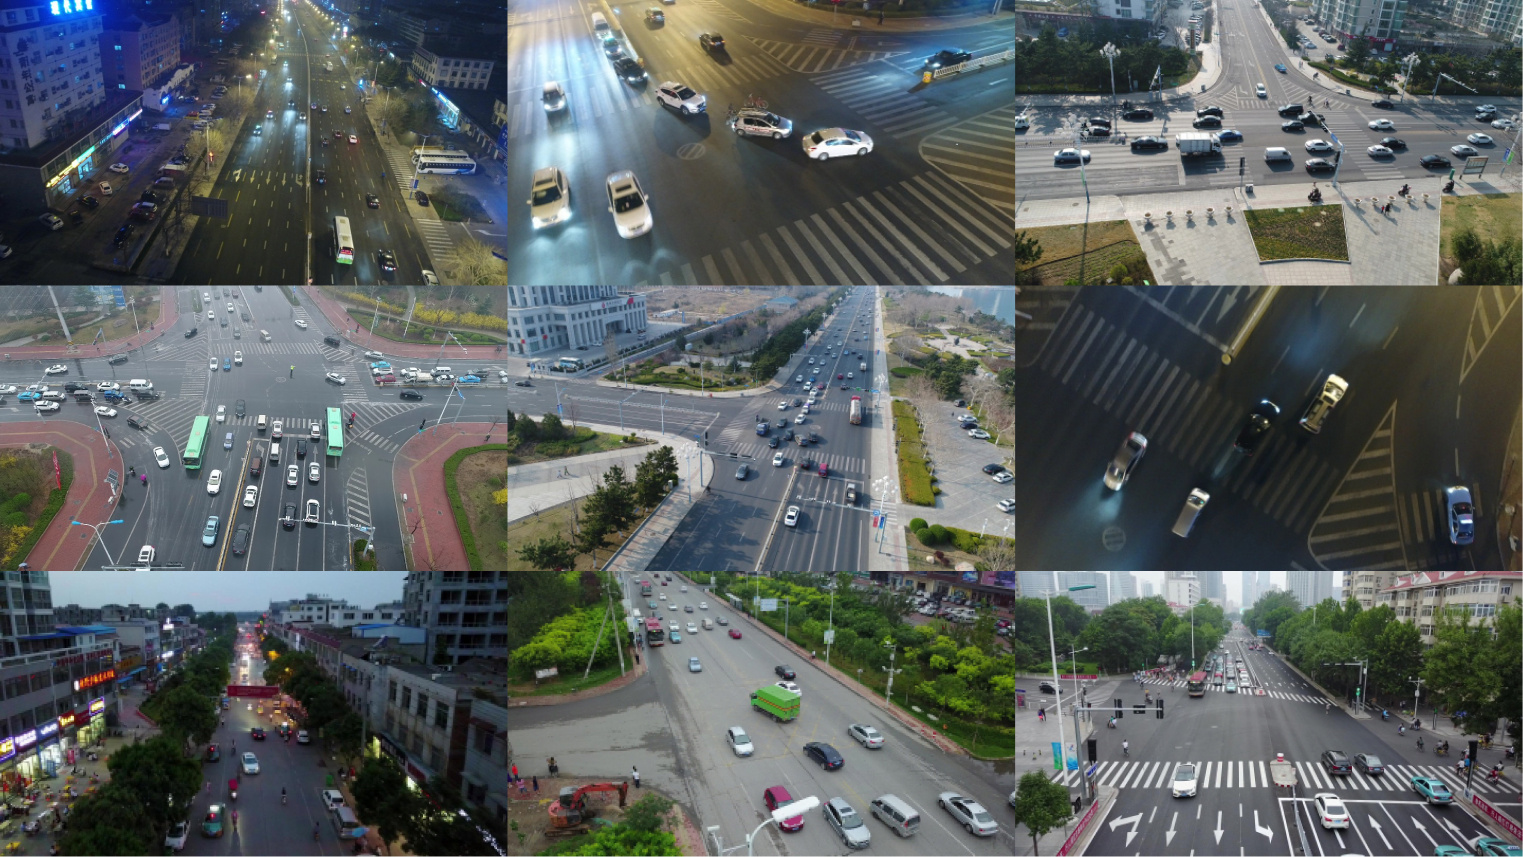
\includegraphics[width=0.85\textwidth]{4-1}
    \caption{Пример выборки кадров из нескольких видео UAVDT}
    \label{img:4-1}
\end{figure}

Датасет был собран командой исследователей из Национального университета Сингапура (NUS) с целью установления стандарта оценки алгоритмов отслеживания объектов в случае сложных сценариев и способствования проведению новых исследований в этой области. Для этого было выполнено аннотирование около 80,000 кадров с помощью 840,000 ограничивающих рамок для 2,700 транспортных средств, как на Рис. \ref{img:4-2}, а также были предоставлены данные о варьирующихся параметрах, таких как высота съемки, погодные условия и точки обзора, краткая информация о которых представлена на Рис. \ref{img:4-3}.

\begin{figure}[ht]
    \centering
    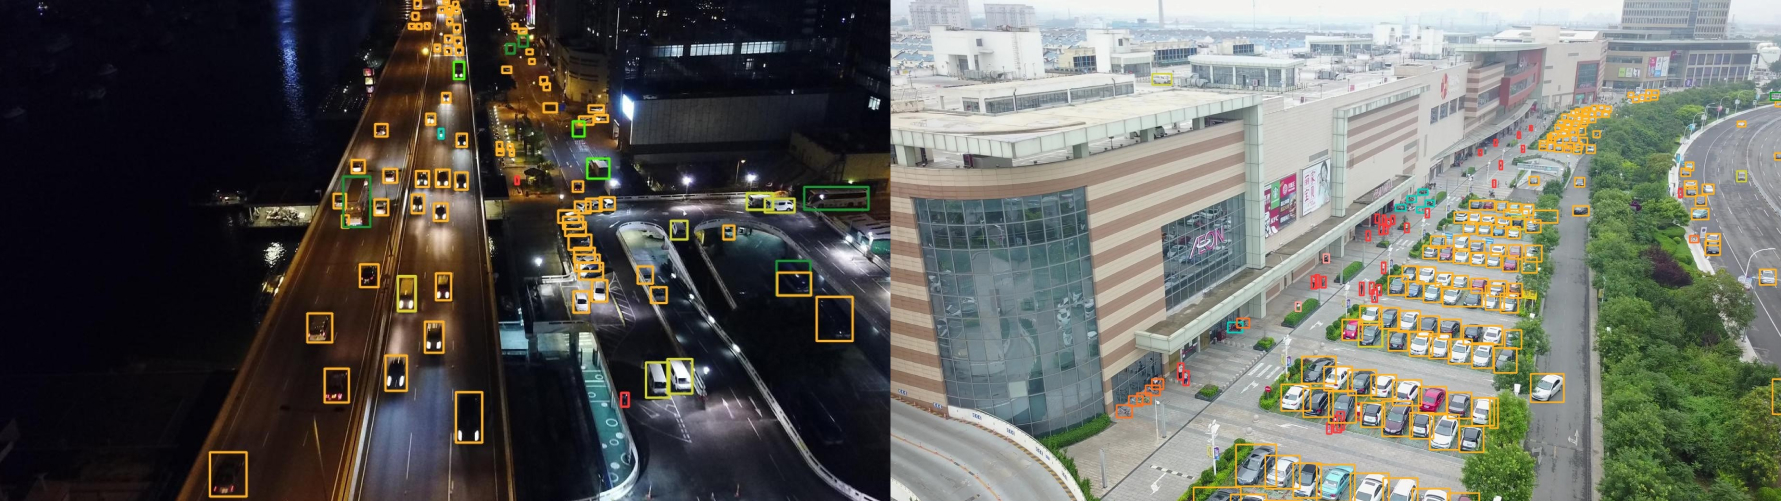
\includegraphics[width=0.85\textwidth]{4-2}
    \caption{Пример аннотированных кадров UAVDT}
    \label{img:4-2}
\end{figure}

\begin{figure}[ht]
    \centering
    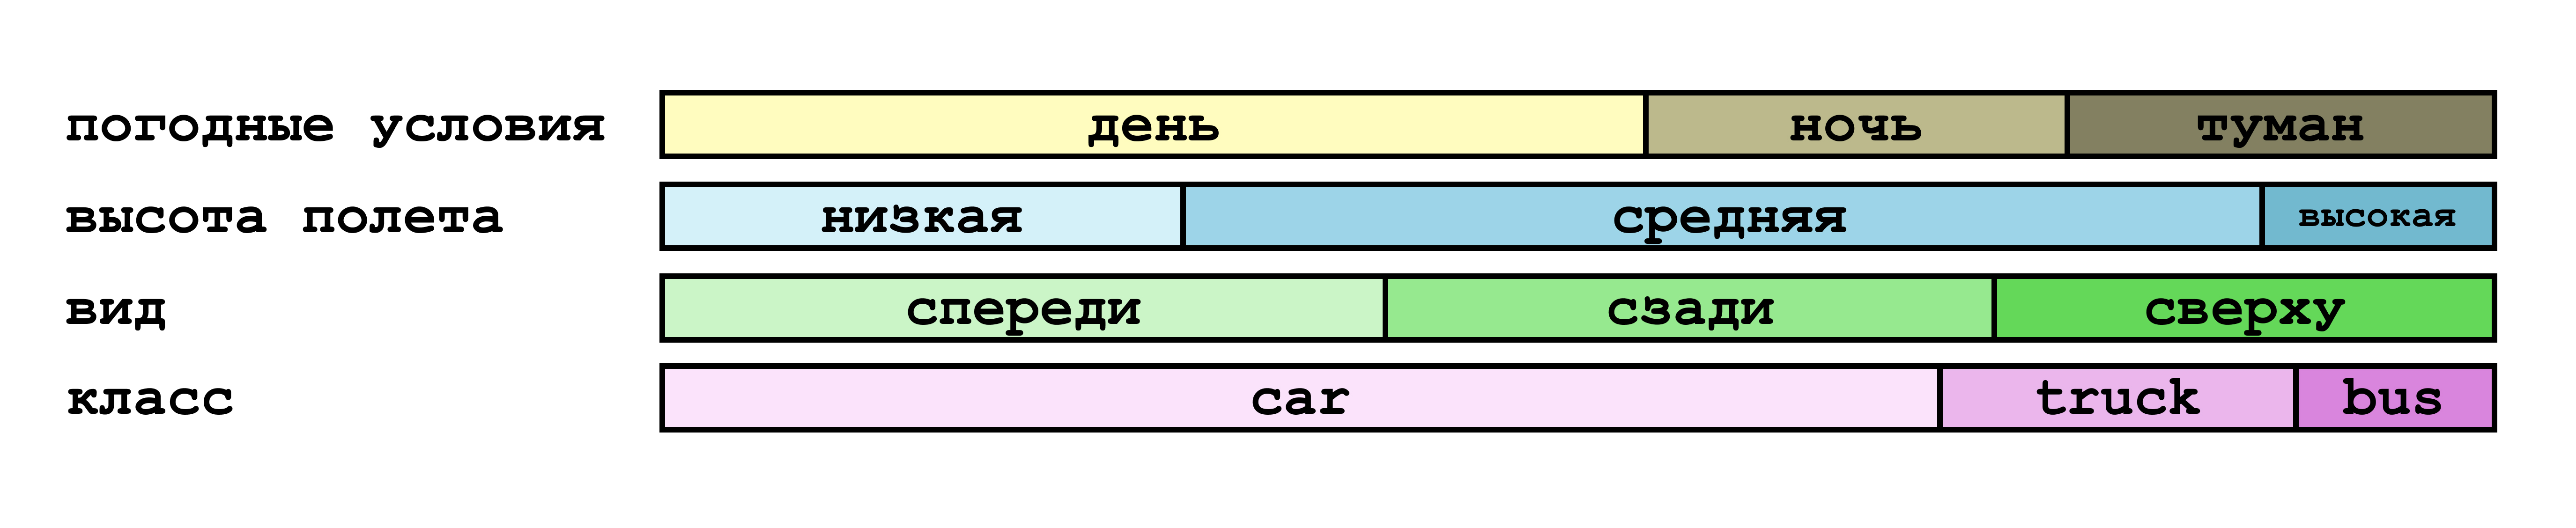
\includegraphics[width=0.85\textwidth]{4-3}
    \caption{Распределение признаков в UAVDT}
    \label{img:4-3}
\end{figure}

Весь датасет подразделяется на 3 задачи: детектирование множества объектов, трекинг одного объекта и трекинг множества объектов. Всего в датасете представлено 3 класса: car, bus и truck, но несмотря на их малое разнообразие, UAVDT обладает более высокой плотностью объектов в кадре, равной 10.52 \cite{4-2}, в сравнении с другими подобными датасетами.
